% Für Bindekorrektur als optionales Argument "BCORfaktormitmaßeinheit", dann
% sieht auch Option "twoside" vernünftig aus
% Näheres zu "scrartcl" bzw. "scrreprt" und "scrbook" siehe KOMA-Skript Doku
\documentclass[12pt,a4paper,titlepage,headinclude,bibtotoc]{scrartcl}


%---- Allgemeine Layout Einstellungen ------------------------------------------

% Für Kopf und Fußzeilen, siehe auch KOMA-Skript Doku
\usepackage[komastyle]{scrpage2}
\pagestyle{scrheadings}
\setheadsepline{0.5pt}[\color{black}]
\automark[section]{chapter}


%Einstellungen für Figuren- und Tabellenbeschriftungen
\setkomafont{captionlabel}{\sffamily\bfseries}
\setcapindent{0em}


%---- Weitere Pakete -----------------------------------------------------------
% Die Pakete sind alle in der TeX Live Distribution enthalten. Wichtige Adressen
% www.ctan.org, www.dante.de

% Sprachunterstützung
\usepackage[ngerman]{babel}

% Benutzung von Umlauten direkt im Text
% entweder "latin1" oder "utf8"
\usepackage[utf8]{inputenc}

% Pakete mit Mathesymbolen und zur Beseitigung von Schwächen der Mathe-Umgebung
\usepackage{latexsym,exscale,stmaryrd,amssymb,amsmath}

% Weitere Symbole
\usepackage[nointegrals]{wasysym}
\usepackage{eurosym}

% Anderes Literaturverzeichnisformat
%\usepackage[square,sort&compress]{natbib}

% Für Farbe
\usepackage{color}

% Zur Graphikausgabe
%Beipiel: \includegraphics[width=\textwidth]{grafik.png}
\usepackage{graphicx}

% Text umfließt Graphiken und Tabellen
% Beispiel:
% \begin{wrapfigure}[Zeilenanzahl]{"l" oder "r"}{breite}
%   \centering
%   \includegraphics[width=...]{grafik}
%   \caption{Beschriftung} 
%   \label{fig:grafik}
% \end{wrapfigure}
\usepackage{wrapfig}

% Mehrere Abbildungen nebeneinander
% Beispiel:
% \begin{figure}[htb]
%   \centering
%   \subfigure[Beschriftung 1\label{fig:label1}]
%   {\includegraphics[width=0.49\textwidth]{grafik1}}
%   \hfill
%   \subfigure[Beschriftung 2\label{fig:label2}]
%   {\includegraphics[width=0.49\textwidth]{grafik2}}
%   \caption{Beschriftung allgemein}
%   \label{fig:label-gesamt}
% \end{figure}
\usepackage{subfigure}

% Caption neben Abbildung
% Beispiel:
% \sidecaptionvpos{figure}{"c" oder "t" oder "b"}
% \begin{SCfigure}[rel. Breite (normalerweise = 1)][hbt]
%   \centering
%   \includegraphics[width=0.5\textwidth]{grafik.png}
%   \caption{Beschreibung}
%   \label{fig:}
% \end{SCfigure}
\usepackage{sidecap}

% Befehl für "Entspricht"-Zeichen
\newcommand{\corresponds}{\ensuremath{\mathrel{\widehat{=}}}}
% Befehl für Errorfunction
\newcommand{\erf}[1]{\text{ erf}\ensuremath{\left( #1 \right)}}

%Fußnoten zwingend auf diese Seite setzen
\interfootnotelinepenalty=1000

%Für chemische Formeln (von www.dante.de)
%% Anpassung an LaTeX(2e) von Bernd Raichle
\makeatletter
\DeclareRobustCommand{\chemical}[1]{%
  {\(\m@th
   \edef\resetfontdimens{\noexpand\)%
       \fontdimen16\textfont2=\the\fontdimen16\textfont2
       \fontdimen17\textfont2=\the\fontdimen17\textfont2\relax}%
   \fontdimen16\textfont2=2.7pt \fontdimen17\textfont2=2.7pt
   \mathrm{#1}%
   \resetfontdimens}}
\makeatother

%Honecker-Kasten mit $$\shadowbox{$xxxx$}$$
\usepackage{fancybox}

%SI-Package
\usepackage{siunitx}

%keine Einrückung, wenn Latex doppelte Leerzeile
\parindent0pt

%Bibliography \bibliography{literatur} und \cite{gerthsen}
%\usepackage{cite}
\usepackage{babelbib}
\selectbiblanguage{ngerman}

\begin{document}

\begin{titlepage}
\centering
\textsc{\Large Vermittlung strömungsphysikalischer Vorgänge im Experiment,
\\[1.5ex] Universität Göttingen}

\vspace*{3cm}

\rule{\textwidth}{1pt}\\[0.5cm]
{\huge \bfseries
  Versuch Flattern  \\[1.5ex]
  Protokoll}\\[0.5cm]
\rule{\textwidth}{1pt}

\vspace*{3cm}

\begin{Large}
\begin{tabular}{ll}
Praktikant: &  Michael Lohmann\\
% &  Felix Kurtz\\
% &  Kevin Lüdemann\\
% &  Skrollan Detzler\\
 E-Mail: & m.lohmann@stud.uni-goettingen.de\\
% &  felix.kurtz@stud.uni-goettingen.de\\
% &  kevin.luedemann@stud.uni-goettingen.de\\
 Versuchsdatum: & 18.1.2016\\
\end{tabular}
\end{Large}

\vspace*{0.8cm}

\begin{Large}
\fbox{
  \begin{minipage}[t][2.5cm][t]{6cm} 
    Testat:
  \end{minipage}
}
\end{Large}

\end{titlepage}

\tableofcontents

\newpage

\section{Einleitung}
Für die Sicherheit eines Flugzeuges ist in erster Linie die Stabilität wichtig.
Ein Effekt, der dabei verhehrend wirken kann, ist das Flattern.
Dies ist ein im schlimmsten Falle selbstverstärkender Effekt, bei dem die Flügel schwingen.
Zahlreiche (auch tödliche) Abstürze sind hierrauf zurückzuführen.

Deshalb ist es wichtig, zu verstehen, wodurch Flattern entsteht und wie man es möglichst vermeiden kann.


\section{Mögliche Lösungen}
Ist die Anströmung schneller, als eine bestimmte kritische Geschwindigkeit $v_\text{krit}$, so schaukelt sich die Schwingung immer weiter auf.
Dies kann geschehen, da die Dämpfung, welche durch Strukturteile des Flügels ausgeübt wird, ab der kritischen Geschwindigkeit durch die Anregung übertroffen wird.
Es ergeben sich die drei Fälle aus Abb. \ref{fig:daempfung}

\begin{figure}[h]
  \centering
  \subfigure[Stark gedämpfter Fall.\label{fig:gedaempft}]
  {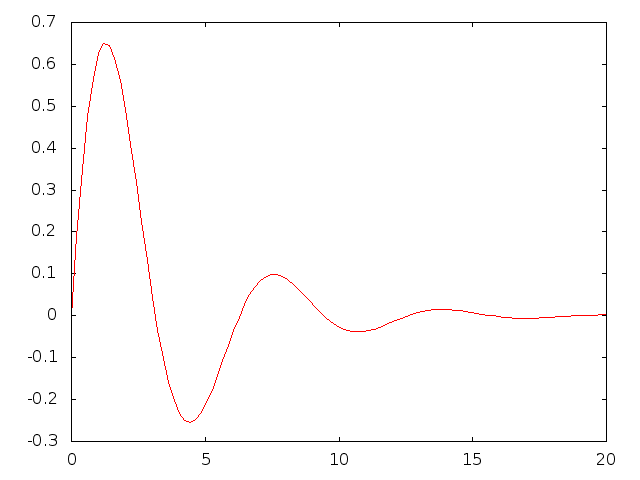
\includegraphics[width=0.30\textwidth]{gedaempft}}
  \hfill
  \subfigure[Dämpfung gerade ausgeglichen an $v=v_\text{krit}$\label{fig:kritisch}]
  {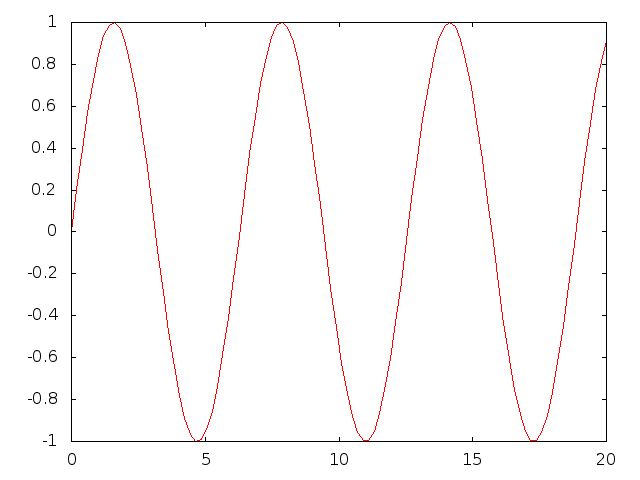
\includegraphics[width=0.30\textwidth]{ungedaempft}}
  \hfill
  \subfigure[Zeitlich verstärkte Anregung mit $v>v_\text{krit}$\label{fig:ueberkritisch}]
  {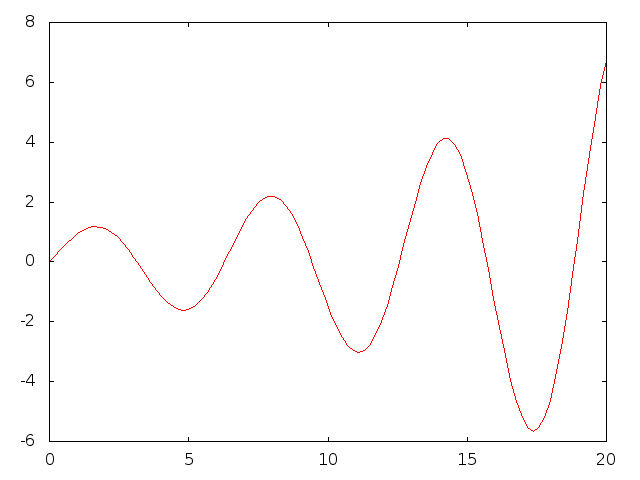
\includegraphics[width=0.30\textwidth]{getrieben}}
  \caption{Auslenkungen im Zeitverlauf bei verschiedenen Geschwingigkeiten.}
  \label{fig:daempfung}
\end{figure}

Das erste Problem ist die schlechte Tarierung der Klappen.
Dies bedeutet, dass die Klappen von alleine nicht in die $0^\circ$-Lage, sondern nach unten fallen.
Dies sorgt jedoch durch Anströmung dafür, dass eine Kraft die Klappen wirkt, welche sie wieder nach oben drückt.
Eine mögliche Lösung ist ein Gegengewicht, was dafür sorgt, dass die Klappe in der Ruhelage nicht ausgelenkt ist.
Dies konnten wir überprüfen, indem wir ein Ruder hatten mit einem verstellbaren Gegengewicht.
Es stellte sich heraus, dass es auch bei deutlich höheren Geschwindigkeiten nicht ins Flattern geriet.

Um genauere Analysen zu machen, was genau für Schwingungen im Flügel auftreten, umströmten wir keinen Flügel mehr mit Klappen, sondern versetzten einen







\end{document}
